\section*{List of Abbreviations}
\label{sec:abbreviations}
\addcontentsline{toc}{section}{List of Abbreviations}

\begin{tabular}{ll}
  {\bf PWM}& Pulse Width Modulation\\
\end{tabular}
\section{Background}
\label{sec:background}

Agricultural Spraying machines are used to apply chemicals to farmland to increase the productivity of the plants.  Fertilizer increases yield by $40\%$ to $60\%.$  If pesticides are not used, yield decreases by $50\%$ to $90\%.$\todo{Dr. Miah, Do we need a reference here?}  To maximize these yields, the correct amount of chemical must be applied to the correct area of the plant or directly to the soil. 
%
\begin{figure}
  \centering
  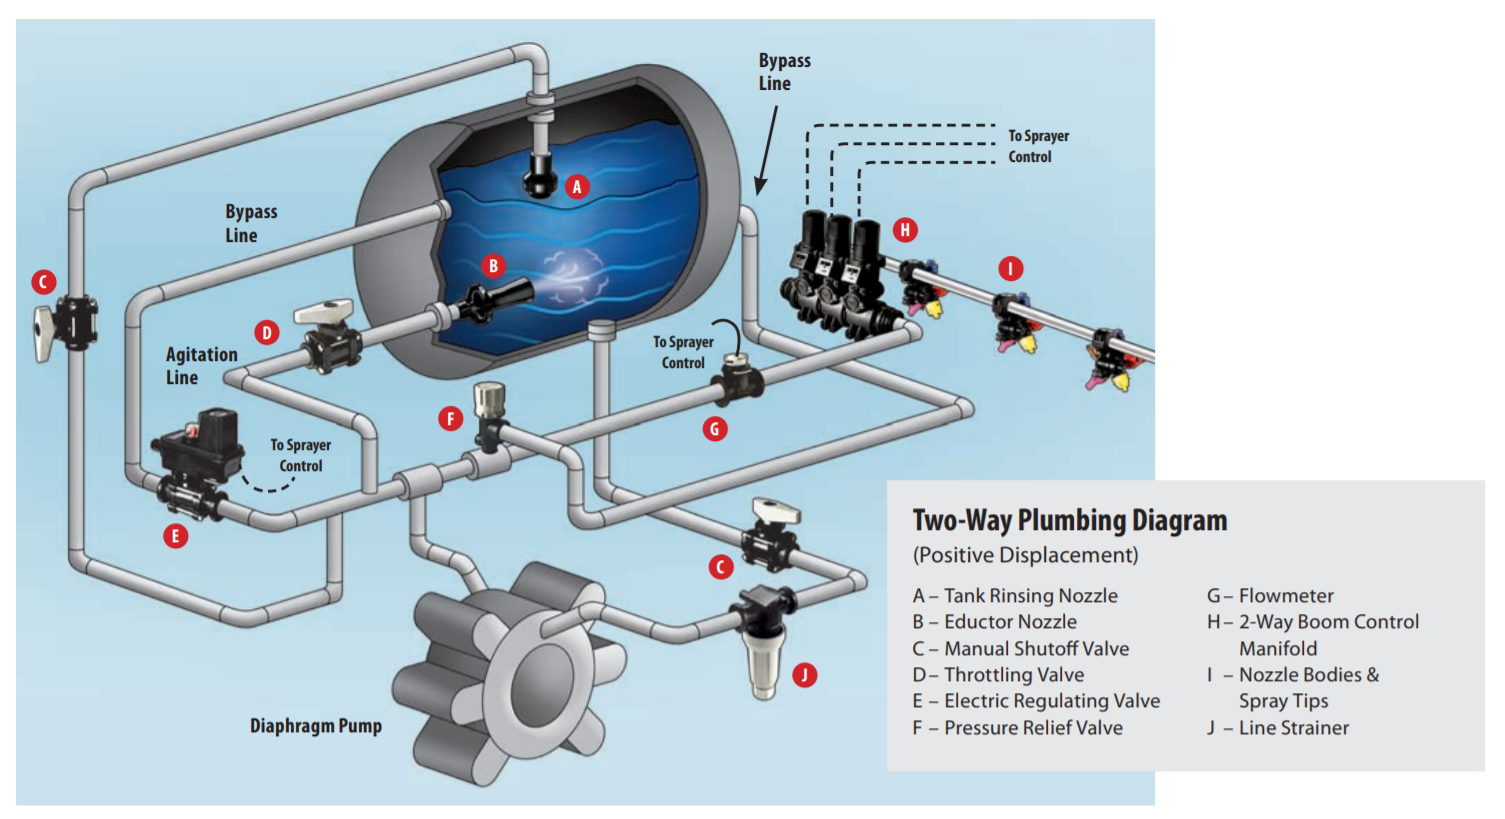
\includegraphics[width=0.7\textwidth]{figs/img/twoWayPlumbingDiagramSrayingMachine}
  \caption{Two-way plumbing diagram of an agricultural srayping machine [Courtesy of TeeJet Technologies].}
  \label{fig:twoWayPlumbingDiagramSrayingMachine}
\end{figure}

A two-way plumbing diagram of an agricultural spraying machine is shown in Figure~\ref{fig:twoWayPlumbingDiagramSrayingMachine}.  Chemical is added to water to the tank of the sprayer to dilute the chemical to the proper concentration. When the pump is engaged, fluid flows from the bottom of the tank to the pump through \textbf{Maunual Shutoff Valve C}, \textbf{Line Strainer J} and into the pump. In some sprayers, the speed of the pump can be changed. Here, fluid can flow in a number of directions depending on the configuration of the Sprayer. 

Fluid can flow back to the tank to agitate or mix the chemical into the water so that sediment does not form at the bottom of the tank.  This is manually changes by moving the position of \textbf{Throttling Valve D}. If too much pressure builds up in the system, \textbf{Pressure Relief Valve F} opens to prevent system damage. The amount of fluid pumped out to the boom can be changed by opening or closing \textbf{Electric Regulating Valve E}. This is typically controlled by an embedded system. The amount of fluid pumped out to the boom is measured by the \textbf{Flowmeter G}.  The flow rate measured by \textbf{Flowmeter G} indicates how much fluid is being applied to the farmland. 

The boom is split into sections containing consecutive groups of nozzles. Boom sections can be turned on and off by\textbf{ Boom Control Manifold H}. Fluid exits the boom from the \textbf{Nozzle Bodies and Spray Tips I}. The mechanics of the nozzles create a spray when exiting the boom. Droplet size if a function of the pressure across the boom.  \textbf{Nozzle Bodies and Spray Tips I} have a solenoid attach that opens or closes the valve as shown in Figure~\ref{fig:SprayPattern} \todo{Image take from web - needs to be remade}.  By applying a PWM signal, we can control the pressure across the boom without impacting the flow rate.
%
\begin{figure}
  \centering
  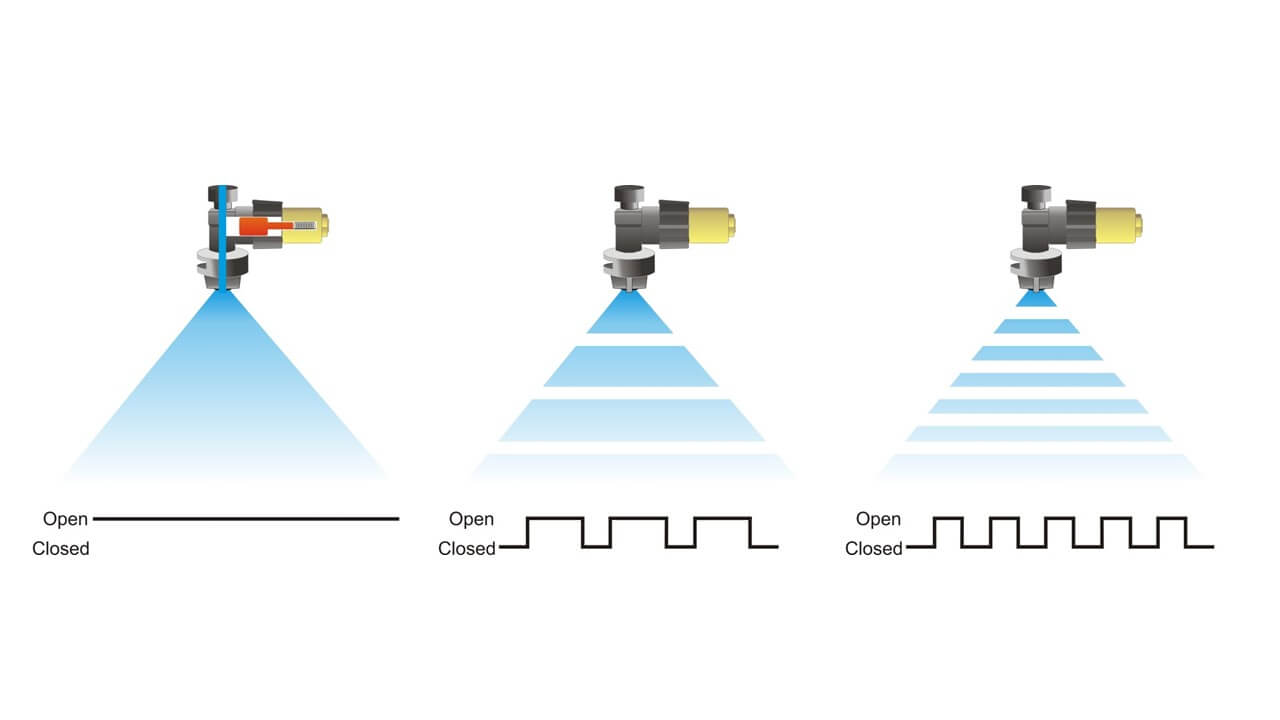
\includegraphics[width=0.7\textwidth]{figs/img/PWM-valve}
  \caption{Nozzle Body Spray Pattern when Applied a PWM Signal.}
  \label{fig:SprayPattern}
\end{figure}


\section{Problem Statement and Objectives}
\label{sec:probl-stat-object}

Farming chemicals are regulated by the government which certifies the chemical for certain droplet sizes. This limits the farmer to how fast the vehicle can drive and apply the correct amount of chemical without an increase in pressure to achieve the same flow rate [L/ha]. In a sprayer application, we have two separate discrete-time feedback control systems to solve these problems:

\begin{enumerate}
\item \textbf{Rate Controller}: this system controls to a desired flow rate [L/ha].  This system ensures the correct amount of fluid is applied to the field.  Target flow is calculated by the prescription for the field, the speed of the vehicle, and the length of the boom. 

\item \textbf{Droplet Size Controller}: this system controls to a constant pressure across the boom of a sprayer.  Droplet size directly correlates to the pressure across the boom. This can be determined from the nozzle’s datasheet (see TeeJet product catalog).  This ensures proper application of the fluid and prevents drift due to atmospheric conditions.  

\end{enumerate}

Flow rate controllers and sprayers can all be manufactured by different companies.  This makes it very difficult to come up 
with a Droplet Size Controller design that will perform on all machines without developing a unique system for every configuration.

Figure~\ref{fig:twoInputTwoOutputDT-ControlSystem} shows the block diagram of a two-input two-output discrete-time control system block diagram, where  $D_2(z),$ $G(z),$ $y_2^{[d]},$ and $y_2$ are assumed to be unknown.
%

\begin{figure}
  \centering
  \begin{tikzpicture}    
      \tikzstyle{every node} = [font=\footnotesize]
      \tikzstyle{block} = [draw, rectangle, fill=blue!15, rounded corners, minimum height=0.5 cm, minimum width=1.0 cm]
      \tikzstyle{sum} = [draw, circle, fill=blue!15];
      \tikzstyle{pinstyle} = [pin edge={to-,thin,black}]
      % Place nodes
      \node[sum](sum){$\sum$};
      \node[block, text width=2 cm, text centered, right of = sum, node distance=3 cm](D1){Droplet Size (Pressure) Controller $D_1(z)$};
      \node[block, text width=2 cm, text centered, below of = D1, node distance=2 cm](D2){Flow Rate Controller $D_2(z)$};
      \node[sum, left of = D2, node distance=2.0 cm](sum3){$\sum$};
      \node[block, text width=1 cm, text centered, right of = D2, node distance=4.5 cm](G){Plant $G(z)$};      
      \node[block, text width=1.5 cm, text centered, below right of = D2, node distance=3.0 cm](H2){Flow meter $H_2(z)$};
      \node[block, text width=1.5 cm, text centered, below of = H2, node distance=2.0 cm](H1){Pressure sensor $H_1(z)$};
      \node[sum, right of = H2, node distance=2 cm](sum2){$\sum$};
      \node[sum, right of = H1, node distance=2 cm](sum1){$\sum$};      

      % Connections 
      \draw[latex-]
      (sum.west)-- node[midway,above]{$y_1^{[d]}$}++(-2*\smgrid,0)node[anchor=east]{Target pressure};
      \draw
      (sum.-165)node[left]{$+$};
      \draw[latex-]
      (sum3.west)-- node[midway,above]{$y_2^{[d]}$}++(-4*\smgrid,0)node[anchor=east]{Target flow rate};
      \draw
      (sum3.-165)node[left]{$+$};
      
      \draw[-latex]
      (sum.east) -- node[midway,above]{$e_1$}(D1.west);
      \draw[-latex]
      (sum3.east) -- node[midway,above]{$e_2$}(D2.west);
      \draw[-latex]
      (D1.east) -| node[near start,above]{$u_1$} (G.north);
      \draw[-latex]
      (D2.15) --++(2*\smgrid,0)|- node[near end,above]{$u_2$}(G.west);
      \draw[-latex]
      (D2.-15) -|node[very near end,right]{$u_3$ (optional)}++(2*\smgrid,-1.5*\smgrid)-| (G.south);

      \draw[-latex]
      (G.20) -- ++(3*\smgrid,0)node[above,right]{$Y_1(z)$};
      \draw[-latex]
      (G.-20) -- ++(3*\smgrid,0)node[below,right]{$Y_2(z)$};
      \draw[-latex]
      ($(G.20) + (1.5*\smgrid,0)$)node[fill,circle,inner sep=1.5pt]{} |- (sum1.east)node[very near end,below]{$+$};
      \draw[-latex]
      ($(G.-20) + (\smgrid,0)$)node[fill,circle,inner sep=1.5pt]{} |- (sum2.east)node[very near end,below]{$+$};

      \draw[-latex]
      (sum2.west) -- (H2.east);
      \draw[-latex]
      (H2.west) -| node[near start,above]{$y_2$} (sum3.south)node[anchor=north east]{$-$}; 
      
      \draw[-latex]
      (sum1.west) -- (H1.east);
      \draw[-latex]
      (H1.west) -|node[near start,above]{$x_1$} (sum.south)node[anchor=north east]{$-$}; 

      \draw[latex-]
      (sum2.south) -- ++(0,-\smgrid)node[below]{$w_2$};
      \draw
      ($(sum2.-90)+(0.05*\smgrid,-0.2*\smgrid)$)node[below,right]{$+$};
      \draw[latex-]
      (sum1.south) -- ++(0,-\smgrid)node[below]{$w_1$};
      \draw
      ($(sum1.-90)+(0.05*\smgrid,-0.2*\smgrid)$)node[below,right]{$+$};
      
      % Layers
      \begin{pgfonlayer}{background}
        \filldraw[fill=yellow!10,draw = blue,dashed,very thick, rounded corners]
        ($(sum.north west) + (-1.9*\smgrid,2*\smgrid)$) rectangle ($(sum1.south east)+(3.5*\smgrid,-2.2*\smgrid)$);
      \end{pgfonlayer}
      \draw
      ($(D1.north)+(\smgrid,\smgrid)$)node[]{\textcolor{blue}{{\bf Discrete-time control system}}};
    \end{tikzpicture}  
  \caption[Two-input, two-output discrete-time control system block diagram.]{Two-input, two-output discrete-time control system block diagram.}
  \label{fig:twoInputTwoOutputDT-ControlSystem}
\end{figure}
%
\begin{table}
  \centering
  \caption{Description of signals used in the control system block diagram shown in Figure~\ref{fig:twoInputTwoOutputDT-ControlSystem}.}
  \label{tab:signalDescription}
  \begin{tabular}{lll}
    \toprule[1.5pt]
    Signal& Description& Unit\\
    \toprule
    $y_1^{[d]}$ & Target pressure & [psi]\\
    $y_2^{[d]}$ & Target flow rate& [GPA]\\
    $y_1$ & Actual pressure & [psi]\\
    $y_2$ & Actual flow rate& [GPA]\\
    %$D_1(z)$ & Pressure controller (transfer function)\\
    %$D_2(z)$ & Flow controller (transfer function)\\
    $u_1$ & Duty cycle to solenoids (limited between $0$ and $100$)& [\%]\\
    $u_2$ & Open/close signal for regulating valve& [V]\\
    $u_3$ & Pump speed (optional)& [rev/min]\\
    %$G(z)$ & Plant model\\
    %$H_1(z)$ & Pressure sensor model (transfer function)\\
    %$H_2(z)$ & Flow meter model (transfer function)\\
    $w_1$ & Pressure sensor noise& [V]\\
    $w_2$ & Flow meter noise& [V]\\
    \bottomrule[1.5pt]
  \end{tabular}
\end{table}
%

{\bf Problem statement:} Develop a control system for the Droplet Size (Pressure) Controller ($D_1(z)$) that can adapt to different plant models and rate controllers.

{\bf Outcomes:}

\textit{TeeJet} expects design of a control system that can: %
\begin{enumerate}
\item adapt to different plant models
\item adapt to different rate controllers 
\end{enumerate}

\textit{Student experience} are expected to learn the following items that pertain to proposed solution:
\begin{enumerate}
\item Design the control system that is ready for implementation
  
\item Conduct computer simulations using MATLAB and Simulink
  
\item Validation and testing using real-time embedded system 
  

\end{enumerate}


\section{Solution Approach}
\label{sec:solutionApproach}

Model-Free Reinforcement Learning Control Approach

The control system of the Droplet Size controller can be simplified as in Figure~\ref{fig:DropletSize-ControlSystem}.
%
\begin{figure}
  \centering
  \begin{tikzpicture}    
      \tikzstyle{every node} = [font=\footnotesize]
      \tikzstyle{block} = [draw, rectangle, fill=blue!15, rounded corners, minimum height=0.5 cm, minimum width=1.0 cm]
      \tikzstyle{sum} = [draw, circle, fill=blue!15];
      \tikzstyle{pinstyle} = [pin edge={to-,thin,black}]
      % Place nodes
      \node[sum](sum){$\sum$};
      \node[block, text width=2 cm, text centered, right of = sum, node distance=3 cm](D1){Droplet Size (Pressure) Controller $D_1(z)$};
      \node[block, text width=1 cm, text centered, right of = D1, node distance=2.5 cm](G){Plant $G(z)$};      
      \node[block, text width=1.5 cm, text centered, below of = D1, node distance=2.0 cm](H1){Pressure sensor $H_1(z)$};
      \node[sum, right of = H1, node distance=2 cm](sum1){$\sum$};      

      % Connections 
      \draw[latex-]
      (sum.west)-- node[midway,above]{$y_1^{[d]}$}++(-2*\smgrid,0)node[anchor=east]{Target pressure};
      \draw
      (sum.-165)node[left]{$+$};
      \draw[-latex]
      (sum.east) -- node[midway,above]{$e_1$}(D1.west);
      \draw[-latex]
      (D1.east) -- node[midway,above]{$u_1$} (G.west);

      \draw[-latex]
      (G.20) -- ++(2.5*\smgrid,0)node[above,right]{$Y_1(z)$};
      \draw[-latex]
      ($(G.20) + (1.5*\smgrid,0)$)node[fill,circle,inner sep=1.5pt]{} |- (sum1.east)node[very near end,below]{$+$};
      
      \draw[-latex]
      (sum1.west) -- (H1.east);
      \draw[-latex]
      (H1.west) -|node[near start,above]{$y_1$} (sum.south)node[anchor=north east]{$-$}; 

      \draw[latex-]
      (sum1.south) -- ++(0,-\smgrid)node[below]{$w_1$};
      \draw
      ($(sum1.-90)+(0.05*\smgrid,-0.2*\smgrid)$)node[below,right]{$+$};
      
      % Layers
      \begin{pgfonlayer}{background}
        \filldraw[fill=yellow!10,draw = blue,dashed,very thick, rounded corners]
        ($(sum.north west) + (-1.9*\smgrid,2*\smgrid)$) rectangle ($(sum1.north east)+(3.5*\smgrid,-2.2*\smgrid)$);
      \end{pgfonlayer}
      \draw
      ($(D1.north)+(\smgrid,\smgrid)$)node[]{\textcolor{blue}{{\bf Discrete-time control system}}};
    \end{tikzpicture}  
  \caption[Single-input single-output discrete-time control system block diagram.]{Single-input single-output discrete-time control system block diagram.}
  \label{fig:DropletSize-ControlSystem}
\end{figure}

Plant will be modeled using a state-space approach:

\begin{align}
  \label{eq:statespaceModel}
\begin{bmatrix}
    x_1[k+1] \\
    x_2[k+1] \\
    x_3[k+1] \\
    x_4[k+1]
\end{bmatrix}&=
\begin{bmatrix}
  a_{11} &  a_{12}&  a_{13}&  a_{14}\\
  a_{21} &  a_{22}&  a_{23}&  a_{24}\\  
  a_{31} &  a_{32}&  a_{33}&  a_{34}\\  
  a_{41} &  a_{42}&  a_{43}&  a_{44}
\end{bmatrix} 
%\label{eq:stateMatrix} 
\begin{bmatrix}
  x_1[k] \\
  x_2[k] \\
  x_3[k] \\
  x_4[k]
  \end{bmatrix}                             
+
%\label{eq:matrixB}
\begin{bmatrix}
    b_{11}\\
    b_{21}\\
    b_{31}\\
    b_{41}
\end{bmatrix}
%\label{eq:inputMatrix}
u_1[k] 
\end{align}
%
where the coefficients of matrices ${\bf A}$ and ${\bf B}$ are unknown.
\highlight{Approximate values for ${\bf A}$ and ${\bf B}$ have been identified using MATLAB's System Identification toolbox as follows:}
%
\begin{align*}
{\bf A}=
\begin{bmatrix}
  0 &  1 & 0 & 0\\
  0 &  0 & 1 & 0\\  
  0 &  0 & 0 & 1\\  
  -0.5724 & 1.551 & -2.193 & 2.106
\end{bmatrix},~~ 
{\bf B}=
\begin{bmatrix}
    -2.4988\times 10^{-4}\\
    -3.6800\times 10^{-4}\\
    -0.0025\\
    -0.0031
\end{bmatrix} 
\end{align*}
%
where the \highlight{sampling time is 50ms.}

\highlight{A typical pressure range is around $55$ [psi] to  $80$ [psi]. A typical flow rate range is around $5$ to $15$ gallons per acre.}

\todo[inline]{Description of the state variables $x_1,$ $x_2, \ldots$ are not available.}


%Flow is typically measured in liters per hectare [L/ha].  This measurement take the length of the boom inconsideration.  For liter per minute [L/min]

%\begin{equation}
%    G(z) = \frac{num}{den}
%\end{equation}


Note that $u_1[k]$ for $k=0,1,2,\ldots,$ is our control signal which will be converted to a PWM signal when sent to the nozzle drivers over the local CAN bus. Let the PWM frequency = $20~[\hertz].$

%$D_1(z)$ & Pressure controller (transfer function)\\
%$D_2(z)$ & Flow controller (transfer function)\\
%$G(z)$ & Plant model\\
%$H_1(z)$ & Pressure sensor model (transfer function)\\
%$H_2(z)$ & Flow meter model (transfer function)\\

%$\dot{x} = Ax + Bu$
%$y = Cx + Du$

The solution will be implemented on an embedded system.

\section{Deliverables}
\label{sec:deliverables}

TBD

\section{Timeline and Milestones}
\label{sec:timeline}



% %
\begin{figure}
  % \begin{sidewaysfigure}
    \centering
    \begin{ganttchart}[hgrid,
      vgrid={*8{black, dotted},*8{black,dotted},*8{black, dotted},*8{black,dotted}},
      title/.style={fill=gray!15,draw=black},
    group/.append style={draw=black, fill=yellow!50},
    group left shift = 0,
    group right shift = 0,
    x unit=.5cm,  % Controls the x-axis grid width of the chart
    y unit title=.8cm,
    y unit chart=.6cm,
    milestone label font=\tiny,
    bar label font=\small, 
    group label font=\normalsize,
    bar/.append style={draw=black,fill=blue},
    bar left shift= 0,
    bar right shift= 0,
    bar height = .7]{1}{20}  % Total number of weeks, from 1 to 20, for example 
    \gantttitle{2020}{20}  % Number of weeks in 2020 
    % \gantttitle{2021}{16}    % Number of weeks in 2021 
    \\
    \gantttitle{July}{4}
    \gantttitle{Aug}{4}
    \gantttitle{Sep}{4}
    \gantttitle{Oct}{4}
    \gantttitle{Nov}{4}\\
    \ganttgroup[progress=25]{{\bf Problem description}}{1}{4}\\
    \ganttbar{Problem analysis}{1}{2}\\
    \ganttbar{Deliverables}{2}{4}\\
%    
    \ganttgroup[progress=25]{{\bf Solution approach}}{2}{8}\\
    \ganttbar{Model-free analysis}{3}{5}\\
    \ganttbar{Reinforcement learning setup}{4}{8}\\
    \ganttgroup[progress=0]{{\bf Implementation}}{8}{16}\\
    \ganttbar{Matlab simulation}{8}{10}\\
    \ganttbar{Simulink implementation}{8}{12}\\
    \ganttbar{Embedded system implementation}{10}{16}\\
    \ganttgroup[progress=0]{{\bf Publication/report}}{16}{20}\\
    \ganttbar{Conference/journal paper}{16}{18}\\
    \ganttbar{Report/workshop/presentation}{16}{20}
  \end{ganttchart}
\caption{Gantt chart showing the project activities from July 2020 to November 2020.}
\label{fig:gantt1}
% \end{sidewaysfigure}
\end{figure}

  
% \end{itemize}
% %
% 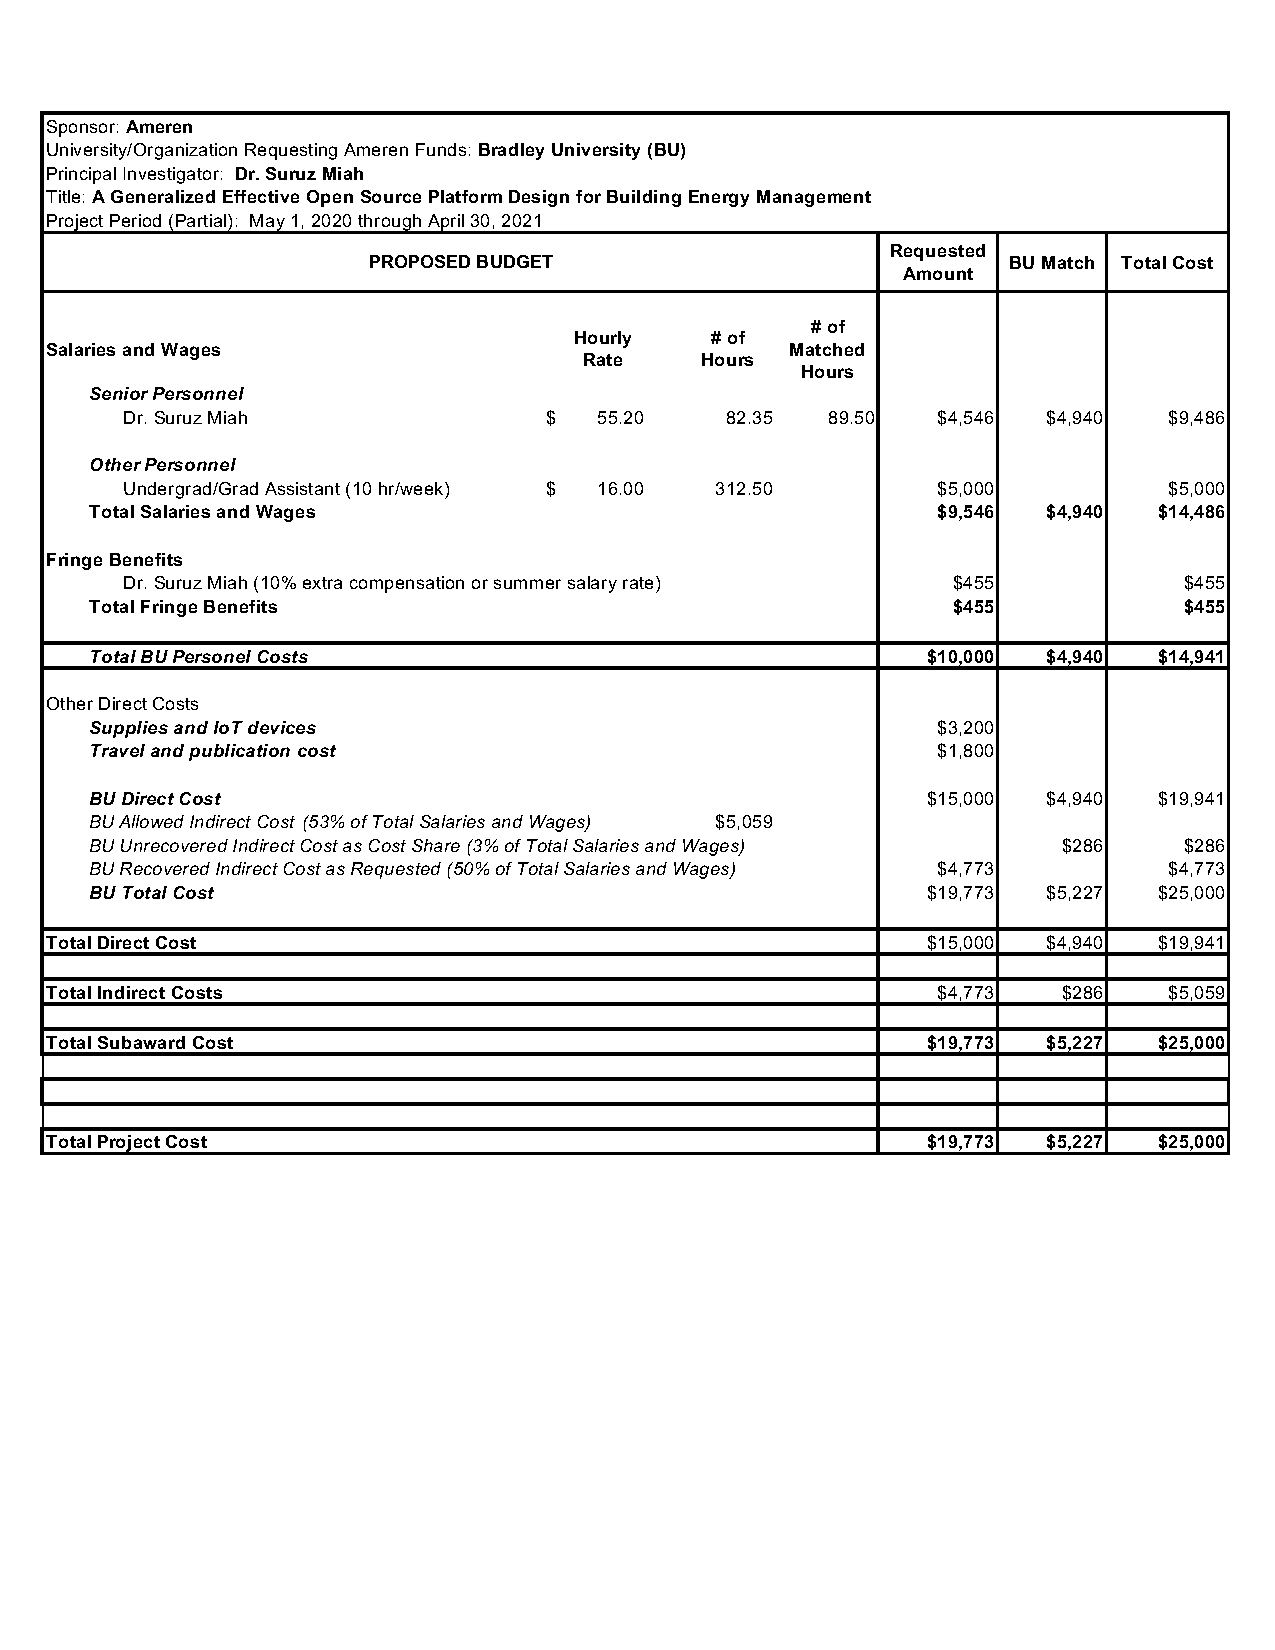
\includepdf[pagecommand={\thispagestyle{fancy}}]{supportingDocs/seedGrantBEMS-AmerenV1.pdf}      

% \subsection{Biographical Sketch of PI}
% PI's biographical sketch is attached in the next page. 
% \includepdf[pages=-,pagecommand={\pagestyle{fancy}}]{supportingDocs/bioSketchMiah.pdf}



%%% Local Variables:
%%% mode: latex
%%% TeX-master: "../mainProposal"
%%% End:
